\useunder{\uline}{\ul}{}
\chapter{Team 5 Agent Design}\label{team_5_agent_design}
\section{Introduction}
\subsection{Leadership Personality}

% FIXME - Fix reference labels
When voted leader with fight power our agent practices utilitarianism [1] and promotes actions that maximizes utility and wellbeing of all agents. For Escape the Dark Pitt, the collective aim is to defeat monsters and clear all levels with remaining population above 60 percent. Hence, we can derive utility being inversely related to damage received by agents and deaths. By prioritizing decisions which will bring upon the greatest utility overall even at his own risk and having a selfless concern for other agents, our agent can also be deemed altruistic. But as completing the game is in our agent's self-interest, it is not pure altruism.

After each monster is defeated, a loot pool is dropped. We believe the loot pool is similar to a Common Pool Resource. All agents have equal opportunities to request for items, deeming the loot pool non-excludable. After an item has been allocated, it is unavailable to other agents, hence the loot pool is also rivalrous in consumption in line with Common Pool Resources. The main difference between the two is the loot pool can be fully depleted each round and fully replenished at the next, while common pool resources generally won't replenish if it is fully depleted. During loot allocation our agent utilizes theory from equity and desert [1] to aim for fairness and distributive justice by having each agent's allocation affected by their contribution. Unlike the health points pool, another common pool resource, agents cannot directly contribute to it. We can determine an agent's contribution by their fight decision as defeating the monster will drop loot, and in turn contribute to the loot pool. Fight decision along with other factors are used to calculate a social network score which will directly impact an agent's ability to be allocated resources per our algorithm.

\subsection{Collective Intelligence}

\begin{figure}[h]
    \centering
    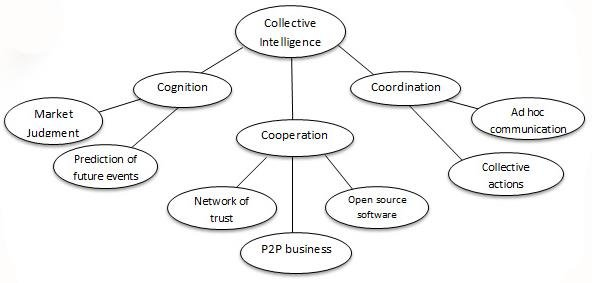
\includegraphics[width=0.63\textwidth]{008_team_5_agent_design/images/Collective-Intelligence-Branches.jpg}
    \caption{Collective Intelligence Branch}
    \label{fig:CQ}
\end{figure}
\begin{flushleft}
\setlength{\parindent}{2em}
As an altruistic agent practicing utilitarianism, our agent aims to improve collective benefit through our own judgement. One way of doing so is to encourage the growth of collective intelligence. Where collective intelligence can be obtained from and have an impact on the following three fields: cognition, corporation, and coordination. We adapt \ref{fig:CQ} \cite{rescher1966} to this game scenario as follows:
\end{flushleft}
\begin{itemize}
  \item Cognition
    \begin{itemize}
        \item Perspectives
            \begin{itemize}
            \item Every agent's perspective on their own status and overall situation - whether they know if they are a popular leader, a helpful peer to the situation, etc. It can be observed from leader status (winning leader election, finishing the leader's term without being overthrown, overthrown). How the majority of other agents are in the social network map, i.e. if only a few agents have a low social network profile, we can deduce that those agents are not welcomed; but if the majority of agents are in a low social network profile, it may be the case that our agent is actually the one that is not welcomed.

            \item Every agent's perspective on other agents can be observed from interaction and information, for example, fight decision (fight intention, defect), proposals, 
            \item Perspective to the environment - agents may over-estimate or under-estimate the monster and the loot market.
            \end{itemize}
        \item Interpretation of the common goal
            \begin{flushleft}
            \setlength{\parindent}{2em}
            Agents can interpret the common goal and make up their own beliefs in different ways. For example, agents may determine the spectrum between altruism and selfishness to be the best strategy of achieving the goal with understanding and deduction.
            \end{flushleft}
            \end{itemize}
  \item Cooperation
    \begin{itemize}
        \item Social Network
                \begin{flushleft}
                \setlength{\parindent}{2em}
                In the cooperation process, every agent can gain knowledge of other agents to form an opinion and decide their future interactions. There exists an underlying social network that connects the agent's communication and interaction in some ways. By discovering this social network our agent can make more effective interactions with other agents.
                
                \end{flushleft}
        \item P2P interactions
                \begin{flushleft}
                \setlength{\parindent}{2em}
                With the existence of the social Network, it can impact the social distance of each P2P interaction, in this case, how likely to send a trading message and how likely to mutually agree on a negotiation. 
                \end{flushleft}
    \end{itemize}
  \item Coordination
    \begin{itemize}
        \item Collective action
                \begin{flushleft}
                \setlength{\parindent}{2em}
                With a common goal, agents can self organise to collectively move towards the goal in some way. Each agent's contribution can have an impact on the whole cohort, voting for example. Individual intelligence is the base of collective intelligence as well as how individual intelligence coordinates. With the leader mechanism and communication mechanism in this game, it gives more opportunities to form collective intelligence through coordination interactions.
                \end{flushleft}
    \end{itemize}
\end{itemize}



\subsection{Agent Trade Personality}

\noindent Our trade strategy extends the Agent’s utilitarian approach and altruistic personality to achieving the collective aim. With this in mind, there is no significance in the weapon or shield we equip if the game is lost. Hence, no concern is given towards the weapon or shield equipped when finally escaping the pit. As each agent has an equal opportunity of receiving loot if they chose to fight, the exclusivity of shields and weapons are low. As we have no concern of our final equipped shield or weapon, the allocation of loot (consumption) to other agents will not subtract from our utility, deeming subtractability to be low. This in turn means that trading is not seen as a common pool resource problem.
\noindent On the contrary, other agents may value their weapon and shield equipped at the end of the game. In other words, trading will benefit other agents as weapon and shield statistics are valued, so the subtractability of weapons and shields would greatly increase in their perspective.
Considering agent’s fight decision as their contribution towards loot, and by coupling trading with fight decision, we can frame this as a common pool resource problem. The common pool resource is sustained through defeating monsters with increasing difficulty to drop new and better items. Our agent takes advantage of this observation and rewards agents with regards to their contribution.

\begin{figure}[htb]
    \centering
    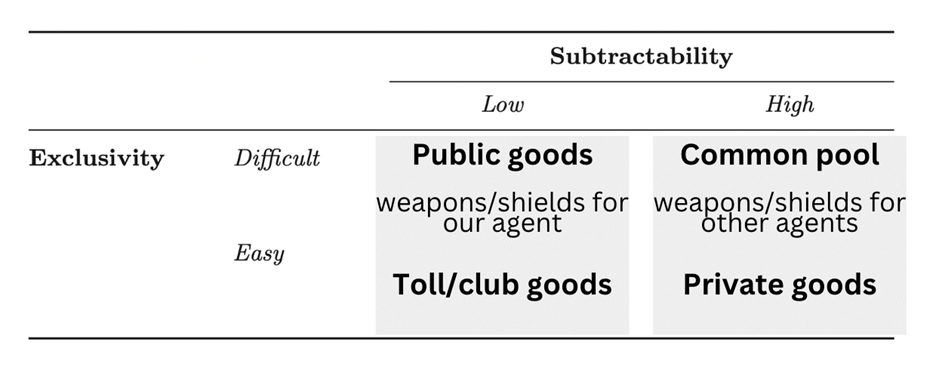
\includegraphics[width=0.60\textwidth]{008_team_5_agent_design/images/13.png}
    \caption{Our agent vs other agent's perspective on trading [1]}
    \label{13}
\end{figure}


\section{Social Network}

We don't want to exclude one's excellence in one field due to short comes in an irrelevant fields.

Here we have agents' algorithm for their fight strategy and the algorithm for their leader duties' functionality potentially written differently.

Hence, we establish two different trusts, which can decouple an agent's strategy quality and leadership goodness. This does not mean the trusts are completely independent, there are still common factors for both of the trusts.The irrelevant features are excluded from one to another.

The agent uses these trusts to summaries features from the left-hand side and contributes to the decision-making of the right-hand side.

Due to the limited size of the game and size of the features, it is sensible to summaries this 2-D personality based on two trust scores

The boundaries for the trust scores are both at $0.2$ and $0.8$ and initial scores at $0.5$, all of the agents will be True Neutral agents at the beginning and will be the majority for most of the game time. When developing the logic, True Neutral agents are included in all of the interactions, although priority will be given to some other personalities, but,
\begin{enumerate}
    \item The prioritised agents are small amount due to a high standards therefore to make sure there is still the majority of the resource that is left with the bigger amount of agents
    \item The accumulated trust addition in a level is less than $0.2$ for each of the scores, therefore it will take at least 2 levels for an agent to gain a personality with priority, which ensures enough interaction has happened or enough information is gained for the agent that we can make a new judgment to its personality. When updating the trust, if there is a trust score exceeding the region of 0-1, the max-min scale is applied to all agents. Under this circumstance, there will be at least one min-scored agent and one max-scored agent that has two different personalities that are not neutral.
\end{enumerate}

\newpage
%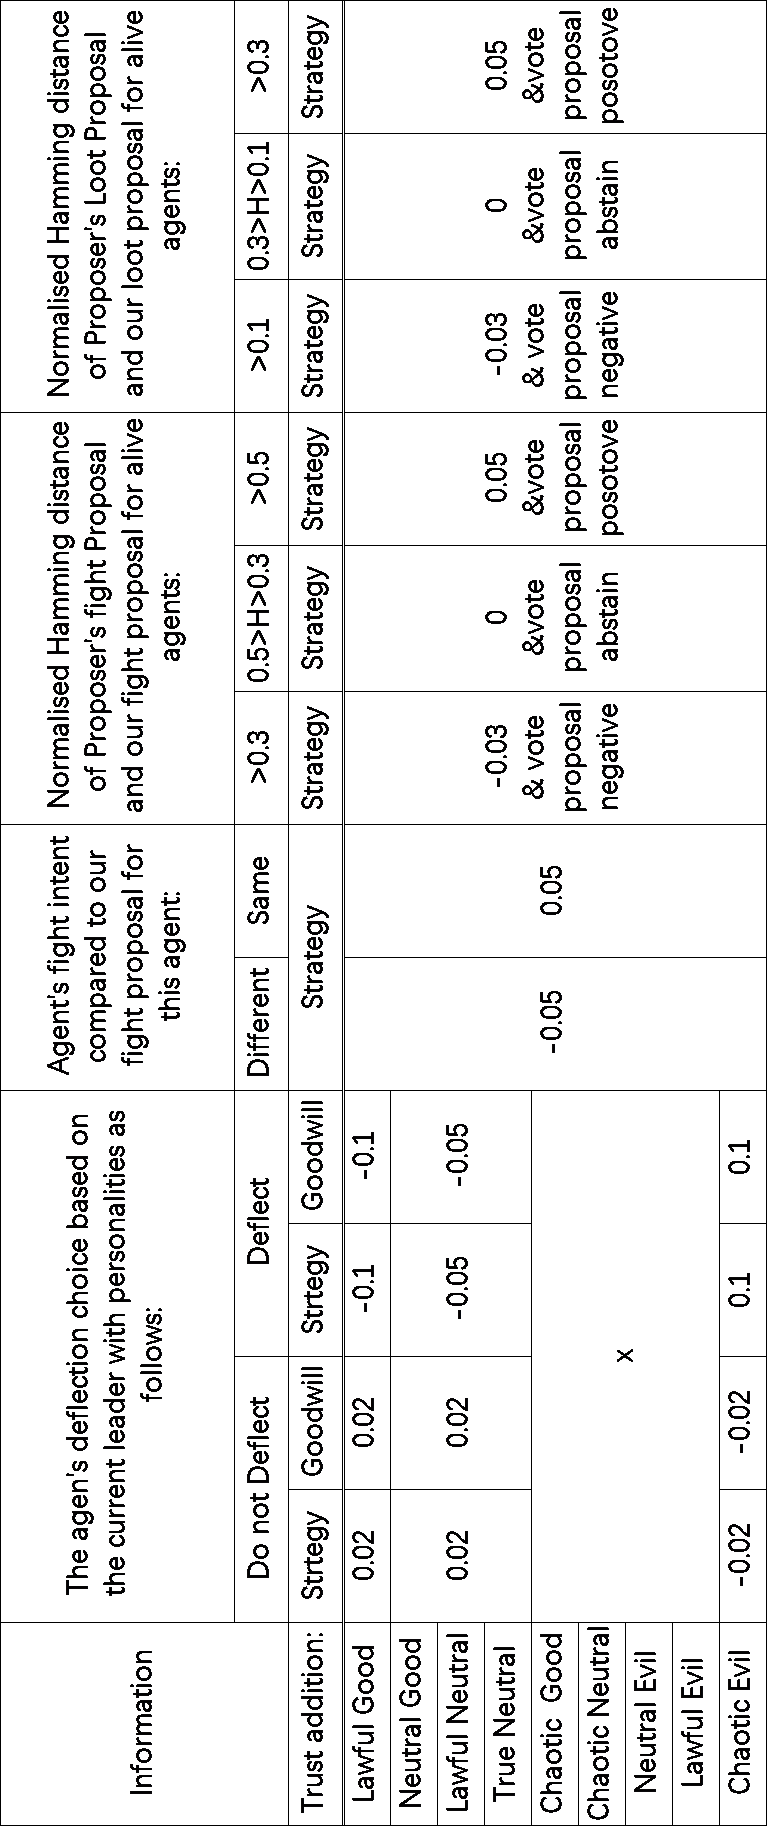
\includegraphics[scale=1]{008_team_5_agent_design/images/Information2Trusts.png}

\begin{figure}[htb]
    \caption{Details of updating trusts regarding different information that can be collected.}
    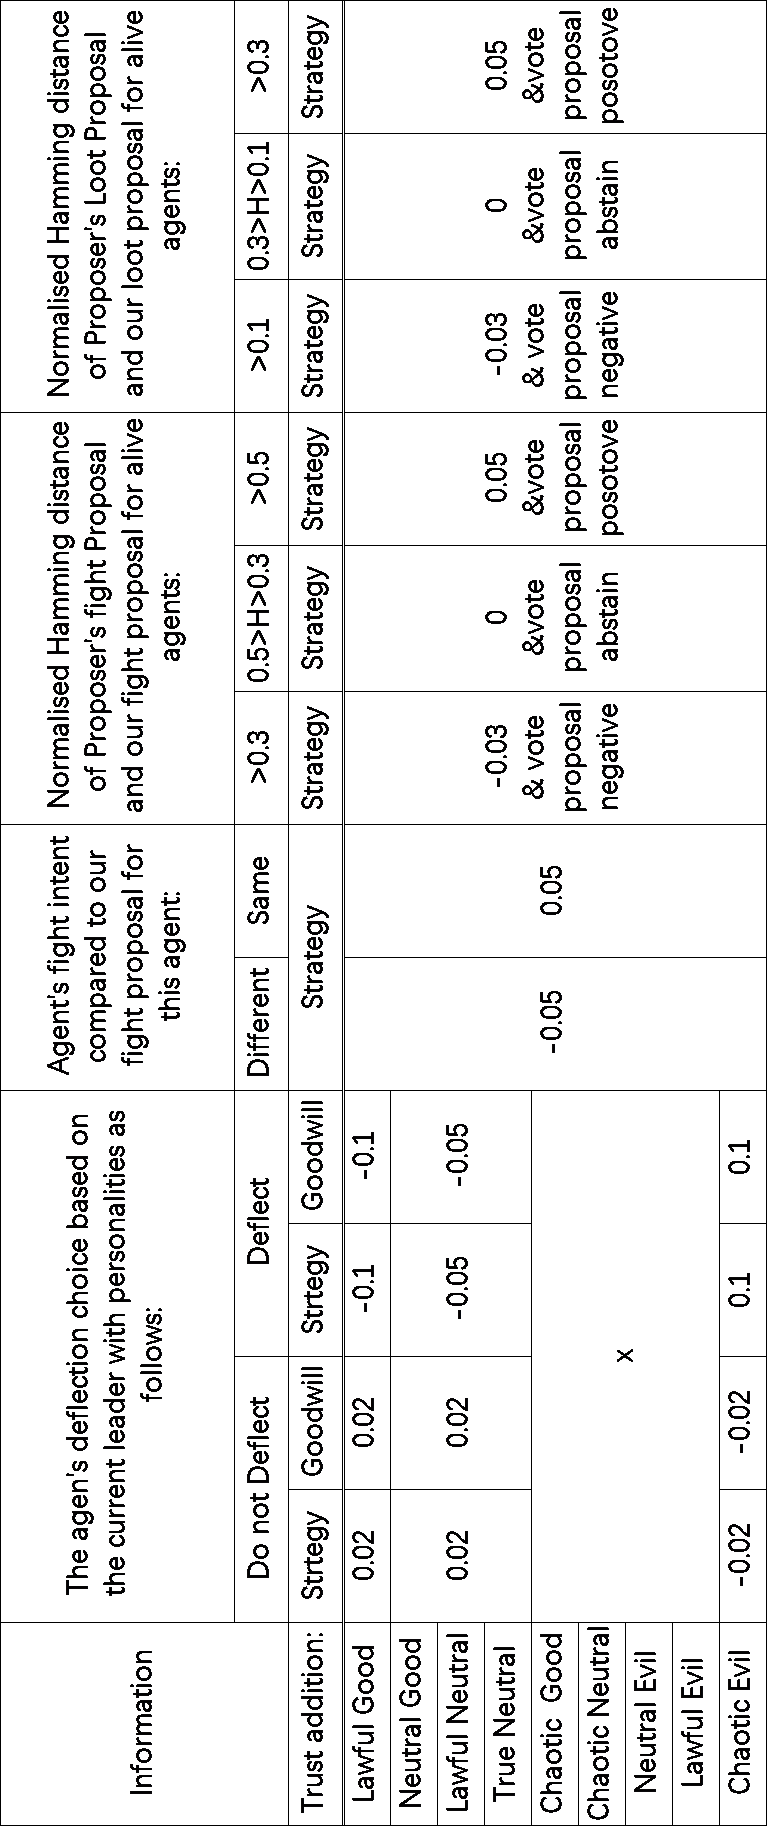
\includegraphics[width=0.60\textwidth]{008_team_5_agent_design/images/Information2Trusts.png}
    \label{fig:Information2Trusts}
\end{figure}
\clearpage

\begin{table}[h!]
    \centering
    \small
    \begin{tabular}{ |c|p{16em}|p{16em}| }
        \hline
        Interaction                       & Loot Resolution                                                                                            & Loot Allocation Proposal                                                                                                 \\
        \hline
        Explaination                      & Extract agents in a conflict with the highest ranked personality as follows and exclude the rest from this & Allocate the loot item with the highest value to the agents with highest ranked personality. Once these gent each got an \\
        \hline
        \multirow{2}{*}{Other Conditions} & Fighting Item                                                                                              & Recovery Item                                                                                                            \\
        \cline{2-3}
                                          & HP != LOW \&\& Stamina != LOW                                                                              & HP == LOW \&\& Stamina == LOW                                                                                            \\
        \hline
        Lawful Good                       & \multicolumn{2}{c|}{1}                                                                                                                                                                                                                \\
        \hline
        Neutral Good                      & \multicolumn{2}{c|}{2}                                                                                                                                                                                                                \\
        \hline
        Lawful Neutral                    & \multicolumn{2}{c|}{3}                                                                                                                                                                                                                \\
        \hline
        True Neutral                      & \multicolumn{2}{c|}{4}                                                                                                                                                                                                                \\
        \hline
        Chaotic Good                      & \multicolumn{2}{c|}{5}                                                                                                                                                                                                                \\
        \hline
        Chaotic Neutral                   & \multicolumn{2}{c|}{6}                                                                                                                                                                                                                \\
        \hline
        Neutral Evil                      & \multicolumn{2}{c|}{7}                                                                                                                                                                                                                \\
        \hline
        Lawful Evil                       & \multicolumn{2}{c|}{8}                                                                                                                                                                                                                \\
        \hline
        Chaotic Evil                      & \multicolumn{2}{c|}{9}                                                                                                                                                                                                                \\
        \hline
    \end{tabular}
    \caption{Other agents' personality impact on our agent's interaction behaviour.}
    \label{table:personality_impact}
\end{table}

\section{Election}

\section{Leadership Logic}
\subsection{Fight Logic}
As mentioned in leadership personality, our agent aims to maximize utility by prioritizing taking the least total damage and deaths when making fight decisions. There are 2 fighting conditions where the level can be passed without taking any damage or deaths. The leader fight algorithm will first check for the following two criterions:

\begin{enumerate}
    \item
          $\sum{\text{Agent Attack}} > \text{Monster Resilience}$

          If the sum of Agent's attack values is greater than monster resilience, we are capable of defeating the monster in one fight round without giving it the opportunity to deal damage.

    \item
          $\sum{\text{Agent Shield}} > \text{Monster Attack}$

          If the sum of Agent's shield values is greater than monster attack, we will receive no incoming damage.
\end{enumerate}

If either criterion is met, the fight decision is determined by minimizing stamina consumption:

\begin{enumerate}
    \item  Agents are ranked according to their attack values. The agent's attack values are summed iteratively starting with the agent with the highest attack value, this is compared against monster resilience for each iteration. Once summed attack is greater than monster resilience, the agent's included in the sum are chosen to attack and all other agents will cower. This ensures we will not deal excessive damage to the monster and waste stamina points that could be utilized in later levels. As agents won't receive damage, their health points are not taken into consideration, meaning low health point agents can still fight.
    \item  Agents are ranked according to their shield values. The agent's shield values are summed iteratively starting with the agent with the highest shield value, this is compared against monster attack for each iteration. Once summed shield is greater than monster attack, the agent's included in the sum are chosen to defend and all other agents will attack in order to defeat the monster with least number of fighting rounds.
\end{enumerate}

If neither criterion can be met, the algorithm will determine whether to prioritize taking the least damage or least deaths by comparing the percentage of surviving agents to a threshold determined by the current level. If percentage of surviving agents is greater than the threshold, the algorithm with prioritize taking the least amount of damage and vice versa. The threshold is set at 90\% for the first 10 levels, then linearly decreases to 60\% (criteria to win game) at the final level.

Once priority is decided, all agents are ranked with respect to health points from high to low. A comparison of the agent's attack and shield value will determine their fight decision, this is done iteratively starting with the agent ranked first. We define total attack as the sum of agent attack values with an attack fight decision, and total shield as the sum of agent shield values with a defend fight decision. Agent's that attack will have 0 shield and agents defending has 0 attack. The first iteration will include only the first agent, such that if the fight decision is attack the total attack would equal to the agent's attack value and shield would be 0. The second iteration will include the first and second ranked agents, this is shown with the figure below:

\begin{figure}[htb]
    \centering
    \includegraphics[width=1\textwidth]{008_team_5_agent_design/images/Rank-all-Agents-by-hp.png}
    \caption{Agents are ranked based on thier health points}
    \label{rankagents}
\end{figure}


Using number of fighting agents, total attack and total shield, the algorithm will determine the estimated damage taken by all agents and expected number of agent deaths. Dividing monster resilience by total attack, we can solve for the number of fighting rounds required to defeat the monster.
\[\text{Fighting Rounds to Kill Monster} \approx \frac{\text{Monster Resilience}}{\text{Total Attack}}=R\]
Using monster attack, total shield, and number of fighting agents we can determine the damage to individual agents per round as:
\[\text{Damage to Individual Agent Per Round} = \frac{\text{Monster Attack}\mathrm{-}\text{Total Shield}}{\text{Number of Fighting Agents} (N)}\ =D_R\]
Therefor total damage received by agents can be calculated by:
\[\text{Total damage received by agents} = D_R \times N \times R = D_T\]
Using $D_R$ we can obtain the damage received by an individual agent to pass the level:
\[\text{Damage received by agent to pass level} = D_R \times  R = D_P\]
And agent deaths are determined by the number of agents with health points lower than $D_P$.

To ensure total attack and total shield values are not skewed, each agent's attack values were scaled 5 times with factors between 0.5 and 2 when determining their fight decision. Continuing our figure example, we can see below in figure how individual agent fight decisions can change.
\begin{figure}[htb]
    \centering
    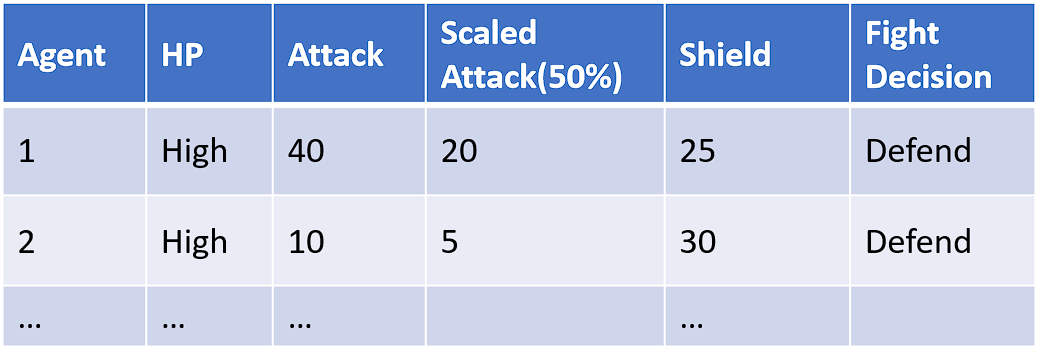
\includegraphics[width=1\textwidth]{008_team_5_agent_design/images/scaled-attack.PNG}
    \caption{Agent attack values are scaled by 50\%}
    \label{scaledattack}
\end{figure}

The scaling factors will give a more comprehensive view for different agent fight decision combinations, hence increasing our likelihood of finding a fight solution that is truly optimal. If all agents are alive, there could be up to 100 iterations for each of the 5 scaled attacks. But by performing each iteration in parallel, we can reduce the execution time and ensure time constraints are met.

If the number of fighting agents exceeds the calculated number of deaths for the iteration, the level is passed. From the iterations that meet this criterion, the one which optimizes for least damage or least deaths are chosen with regards to our predetermined priority. The algorithm will finally return a fight decision map reflecting our best fight solution for the current level.


\subsection{Manifesto}



\section{Fight Logic}
To pass the fighting game as an individual, we want our agent to have the ability to learn within a dynamic environment, where consequences could be introduced via an agent itself or other agents' actions. Learning in this case means to acquire a bank of knowledge and update them throughout time, in order to help fighting the monsters.

\subsection{Fight decision: Q learning}
The fighting stage from an individual agent's point could be viewed as a Markov Decision Process, where from the current state, an agent could have certain probability to transit into another state (new or same), by performing one of the three fighting actions, Attack / Defend / Cower. Depends on whether the agent end up in a better or worse state, it receive some corresponding reward which will cause it to like or dislike the action just being performed.

The state space is designed based on the health, stamina, attack and defence of an agent. Health and stamina are categorised relative to their initial value, so for agent with initial health of 1000, the \textit{Low} category is always $\leq 300$. However, the attack and defence are categorised relative to all other observable agents, for representing potential roles in a population. An agent could be a master fighter (\textit{Master}) when it's attack value is greater than most of the population, or it could be an elder or child (\textit{Weakee}) who's not that good at fighting.

\begin{table}[!ht]
    \centering
    \begin{tabular}{|l|l|l|l|}
        \hline
        \begin{tabular}[c]{@{}l@{}}Health \\ (to init health)\end{tabular}                      & \begin{tabular}[c]{@{}l@{}}Stamina \\ (to init stamina)\end{tabular}                    & \begin{tabular}[c]{@{}l@{}}Attack \\ (to observable agents)\end{tabular}                   & \begin{tabular}[c]{@{}l@{}}Defence \\ (to observable agents)\end{tabular}                  \\ \hline
        \textit{\begin{tabular}[c]{@{}l@{}}Low\\ hp \textless 30\%\end{tabular}}                & \textit{\begin{tabular}[c]{@{}l@{}}Low\\ ap \textless 30\%\end{tabular}}                & \textit{\begin{tabular}[c]{@{}l@{}}Weakee\\ AT \textless 25\%\end{tabular}}                & \textit{\begin{tabular}[c]{@{}l@{}}Weakee\\ SH \textless 25\%\end{tabular}}                \\ \hline
        \textit{\begin{tabular}[c]{@{}l@{}}Mid\\ 30\% \textless hp \textless 60\%\end{tabular}} & \textit{\begin{tabular}[c]{@{}l@{}}Mid\\ 30\% \textless ap \textless 60\%\end{tabular}} & \textit{\begin{tabular}[c]{@{}l@{}}Ordina\\ 25\% \textless AT \textless 75\%\end{tabular}} & \textit{\begin{tabular}[c]{@{}l@{}}Ordina\\ 25\% \textless SH \textless 75\%\end{tabular}} \\ \hline
        \textit{\begin{tabular}[c]{@{}l@{}}High\\ 60\% \textless hp\end{tabular}}               & \textit{\begin{tabular}[c]{@{}l@{}}High\\ 60\% \textless ap\end{tabular}}               & \textit{\begin{tabular}[c]{@{}l@{}}Master\\ 75\% \textless AT\end{tabular}}                & \textit{\begin{tabular}[c]{@{}l@{}}Master\\ 75\% \textless SH\end{tabular}}                \\ \hline
    \end{tabular}
\end{table}
\begin{figure}[!h]
    \centering
    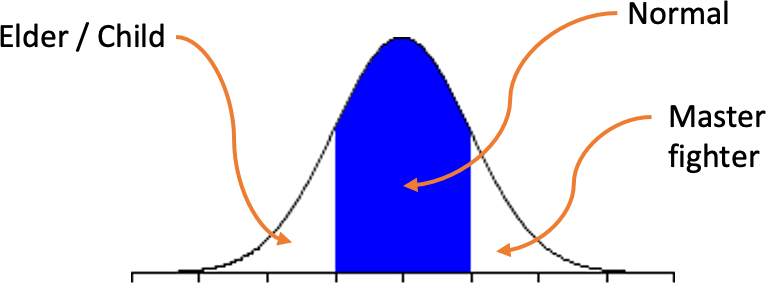
\includegraphics[width=0.6\textwidth]{008_team_5_agent_design/images/state_normal_distro.png}
    \caption{Assumed normal distribution of attack / defence roles.}
    \label{fig:state_normal_distro}
\end{figure}
\noindent
So in total there's 81 different states, where the health / stamina categories are equally separated; the attack / defence categories are separated assuming normal distribution, so extremes are less common and are valuable to treat differently.

In terms of decision, our agent utilise the Q learning algorithm, where each agent keeps a table of Q values as their utilities toward the fighting actions at a given state (a state-action pair), these Q values are updated throughout the game according to feedback (rewards) after each fighting round.

Updates rule:
\begin{center}
$Q(S,A) \leftarrow Q(S,A) + \alpha(R(S^+) + \gamma \max\limits_{A^+} Q(S^+,A^+) - Q(S,A))$
\end{center}
\noindent
Where $Q(S,A)$ is the $Q$ value for a state($S$)-action($A$) pair; $R(S^+)$ is the reward received at the arrived new state, right now it's simply based on the percentage health loss / gain of an agent; $\gamma \max\limits_{A^+} Q(S^+,A^+)$ tries to reflect the potential future reward (in long term), propagate out with a decay rate $\gamma$; $\alpha$ is a learning rate determine how significant each update could be.

The key characteristics of Q learning is that it doesn't really need the state transition probabilities to solve a MDP; also it take in account of the long term effect of an action from a state by the $\gamma \max\limits_{A^+} Q(S^+,A^+)$ term.

Higher Q value for a state-action pair makes it more favourable for an agent to follow. So the strategy for an agent is to go for an action with the highest Q value at the current state, for exploiting its knowledge, but at the same time also allow some random deviation from that to explore the unknowns.

\subsection{Fight proposal: best self-experience}
As the exact opposite to making fight decision, which one has to answer the question ``what's the most promising action to do in such situation", making fight proposal to the others would be to answer the question ``what's the most promising situation to be in if one wants to conduct such action". So in our agent's case, it would be finding the state associated with the highest Q value for a given action.

\begin{figure}[!h]
    \centering
    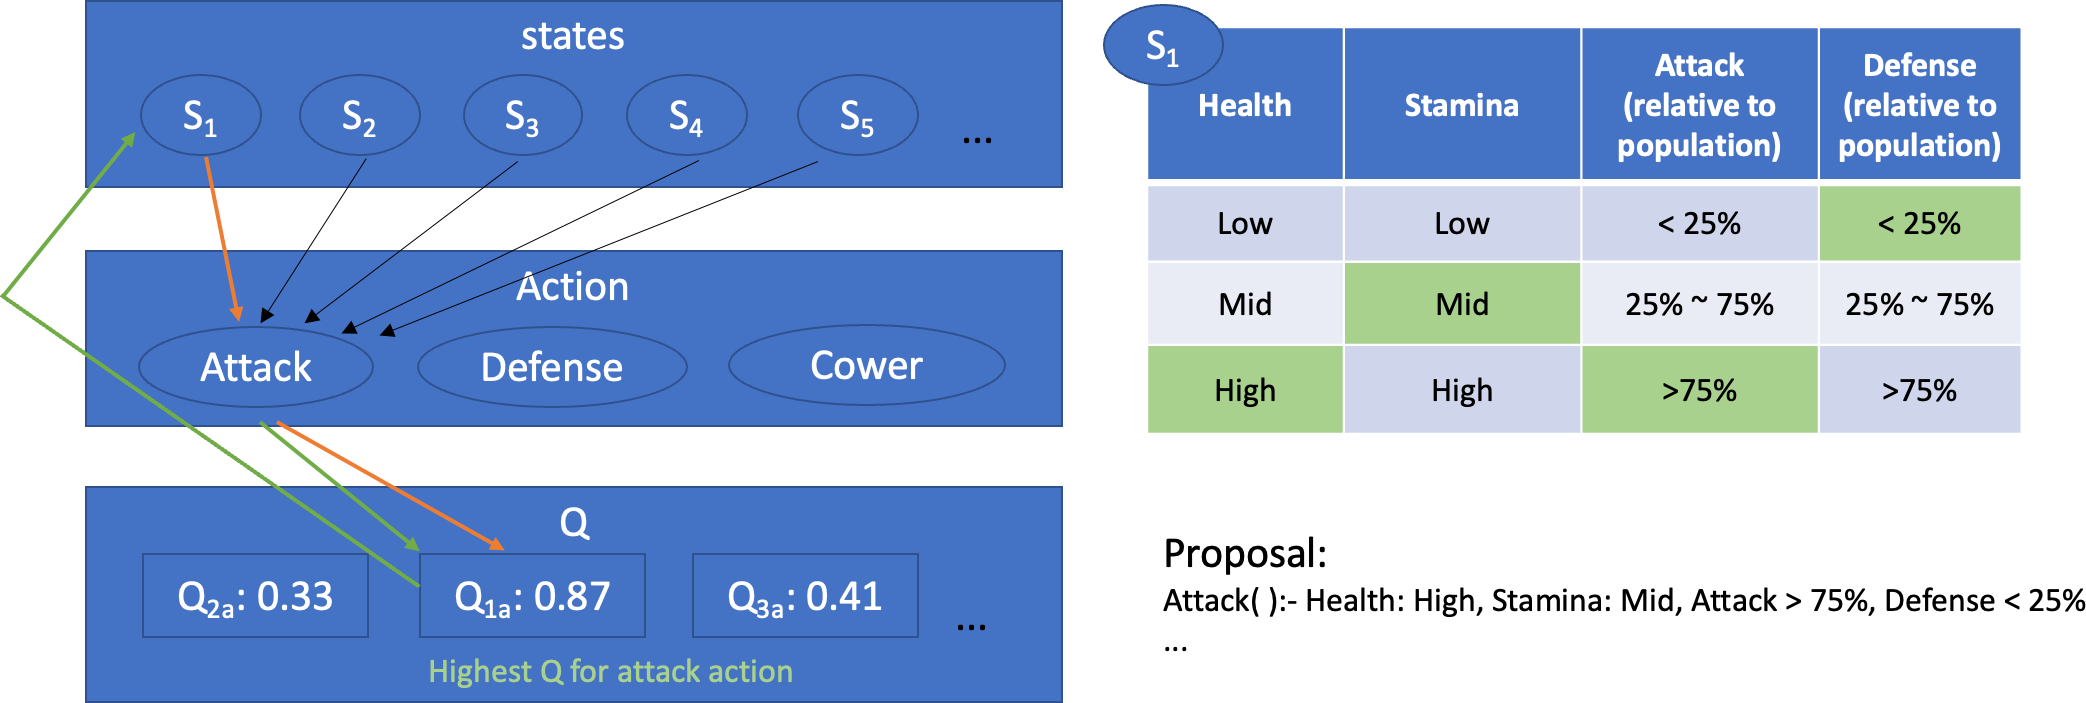
\includegraphics[width=1\textwidth]{008_team_5_agent_design/images/proposal_from_qtable.png}
    \caption{Proposing the most promising state for an action from the Q table}
    \label{fig:proposal_from_qtable}
\end{figure}

While every agent proposes the best strategy according to their self-experience, and all those proposals go to the leader, then depends on how the leader decided to board-cast the appropriate proposal(s) for the group, this could be seen as a process of trying to achieve knowledge aggregation.

\section{Election}
The election stage is setup so that, each of the $N$ agents need to vote for one or more of the other $N-1$ agents. Our agent is designed to produce a trust value $T_{lead}$ for every other agents, it aims to use this social capital to simplify the process of choosing the leader, without explicitly examining other's leader functions.

\subsection{Event-Recency dependent trust}
The trust is designed to be event and recency dependent, which means the recent event of an agent have more importance than those which are long time ago. More precisely defined as:
\begin{center}
$\qquad T(a,b) \leftarrow \gamma \cdot T(a,b) + v(r)$   
\end{center}
Where $T(a,b)$ is the trust of agent $a$ toward agent $b$; $gamma$ is a decay factor to reduce the effect of past memory; $v(r)$ is the rating for an specific event $r$ that happened, typically related to health loss / gain of $a$ and death among the population.

The reason for making past memory become less important throughout time, is to avoid forming stereotype on leading strategies and to preserve diversity, accounting the possibility where one particular leading strategy might not be suitable at one time, but might be suitable for another time.

\subsection{Leader trust estimation}
Since it's not possible to get event feedback for how an agent is going to lead unless this agent is elected to be the leader, which tend to be infrequent, so we designed an estimation for the leader trust combining an agent's normal performance and it's performance when it did act as the leader.
\begin{center}
$T_{lead}^{t+1} = \alpha \cdot T_{lead}^t + \beta \cdot T_{normal}^t$    
\end{center}
So in fact each agent need to keep two trust record for other agents, $T_{normal}$ for whether an agent is doing well on an individual level, and $T_{lead}$ for whether an agent is doing well on a group level. They are then combined to produce a estimation on how trust worthy an agent is to become the new leader, typically in a ratio of $\alpha=0.9, \beta=0.1$ for making past leading experience more significant.

\section{Trading Logic}

\noindent Since each trading round is limited to five messages, choosing which agents to trade with is vital. The leader fight logic is used in our agent’s trade strategy for every decision made. We use the outputted optimal fight decision map to filter out agents that will not likely fight in the following round. Agents predicted to either attack or defend will be prioritised as potential trade candidates. If our own agent is cowering for the following round, agents fighting will be offered our best weapon or shield. This is to ensure the best equipment are always utilized to maximise our chance to escape the pit and achieve the collective goal.

\noindent Our trading strategy will also prioritise agents having a positive or neutral strategy trust over agents with lower trust scores to penalise agents that either defected from their fight decision or are selfish in trades. The combination of agent trust and agent fight actions will reward and encourage agents to contribute towards the common pool resource.

\noindent An issue considered when choosing trade partners was if our policy was deterministic, such that our agent always requested from cowering agents with the best shield or weapon, all team 5 agents initialized within the game would have clashing trade requests. To resolve this issue, our agent searches for trade partners through random starting positions within the agent map and checks iteratively if agents meet our trade criteria of cowering and having a better weapon or shield. A trade request will sent to the first agent that meets our criteria.


\section{Experiment}

\subsection{Leader Fight Logic}
The leader fight logic's execution time was tested to ensure it is within the time limit of 0.5 seconds.

\begin{figure}[htb]
    \centering
    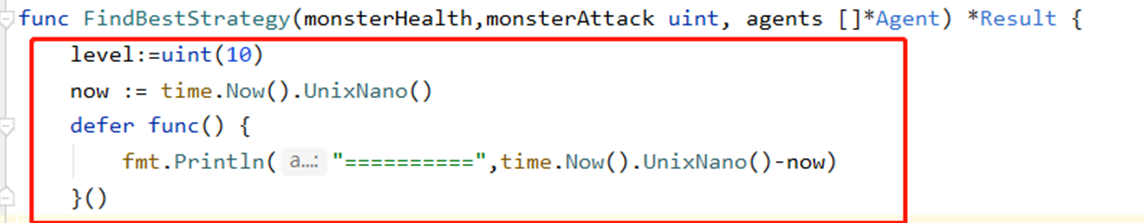
\includegraphics[width=0.7\textwidth]{008_team_5_agent_design/images/10.png}
    \caption{Measuring execution time}
    \label{testingexecutiontime}
\end{figure}

\begin{figure}[!ht]
    \centering
    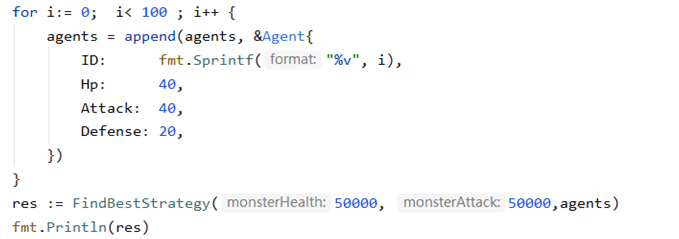
\includegraphics[width=0.7\textwidth]{008_team_5_agent_design/images/11.png}
    \caption{Initialising Agent and Monster}
    \label{initialisingagentandmonster}
\end{figure}

Some results are shown below, execution time is labelled with consumer in units of nano seconds.

\begin{figure}[!ht]
    \centering
    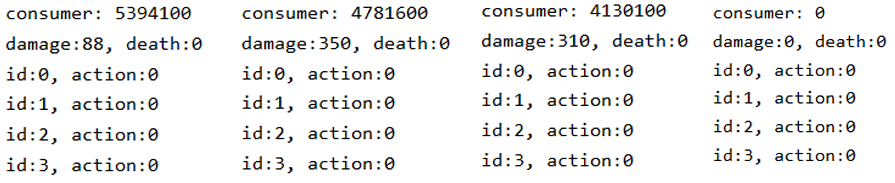
\includegraphics[width=0.7\textwidth]{008_team_5_agent_design/images/12.png}
    \caption{Execution time test results}
    \label{executiontimetestresults}
\end{figure}

All trials had execution time under 0.01 seconds and well below the time limit.

\subsection{Team 5 vs. Random}
Figure \ref{fig:Team5vsRandom} is a comparison between our team's agent vs. the random agent. With two small tweaks are done to the game engine in order to make the comparison under the same controls.

\begin{enumerate}
    \item Turned off HP pool donation: \\
    The current HP pool donation mechanism is way unbalanced and will become a dominated strategy if used, which causes agents to be able to skip all levels until they can't donate health anymore, this prevents all designs on fighting decision or leader function to be relevant.
    \item Stamina regeneration increased: \\
    As on the demo section, the unbalance stamina regeneration is mentioned, where after examining, the original game only regenerate 1 stamina ($0.05\%$ to initial health) per time, so for a more sensible game run, the stamina regeneration is changed to 100 ($5\%$ to initial health) per time.
\end{enumerate}

\begin{figure}[!ht]
    \centering
    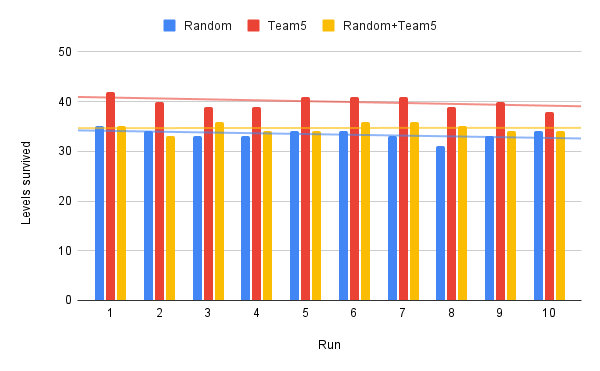
\includegraphics[width=0.8\textwidth]{008_team_5_agent_design/images/Team5vsRandom.png}
    \caption{Game run with 100 Team 5 agents (red); 100 Random agents (blue); 50 Team 5 agents and 50 Random agents (yellow).}
    \label{fig:Team5vsRandom}
\end{figure}

In average our agent could survive 5 more levels then the random agent, with it's own kind. But when playing with half of the population being another kind, the levels survived will only be marginally better than the random agents. This might because the random agents do not keep trust record (no social capital), so the advantage of using social capital to effectively elect leader or appropriating loot is broken.

\subsection{Proposal, trust and knowledge aggregation}
It will be interesting to investigate the effect of allowing agents to propose what they think is the best, also how that might effect leading and whether it helps to do knowledge aggregation.

\begin{figure}[!ht]
    \centering
    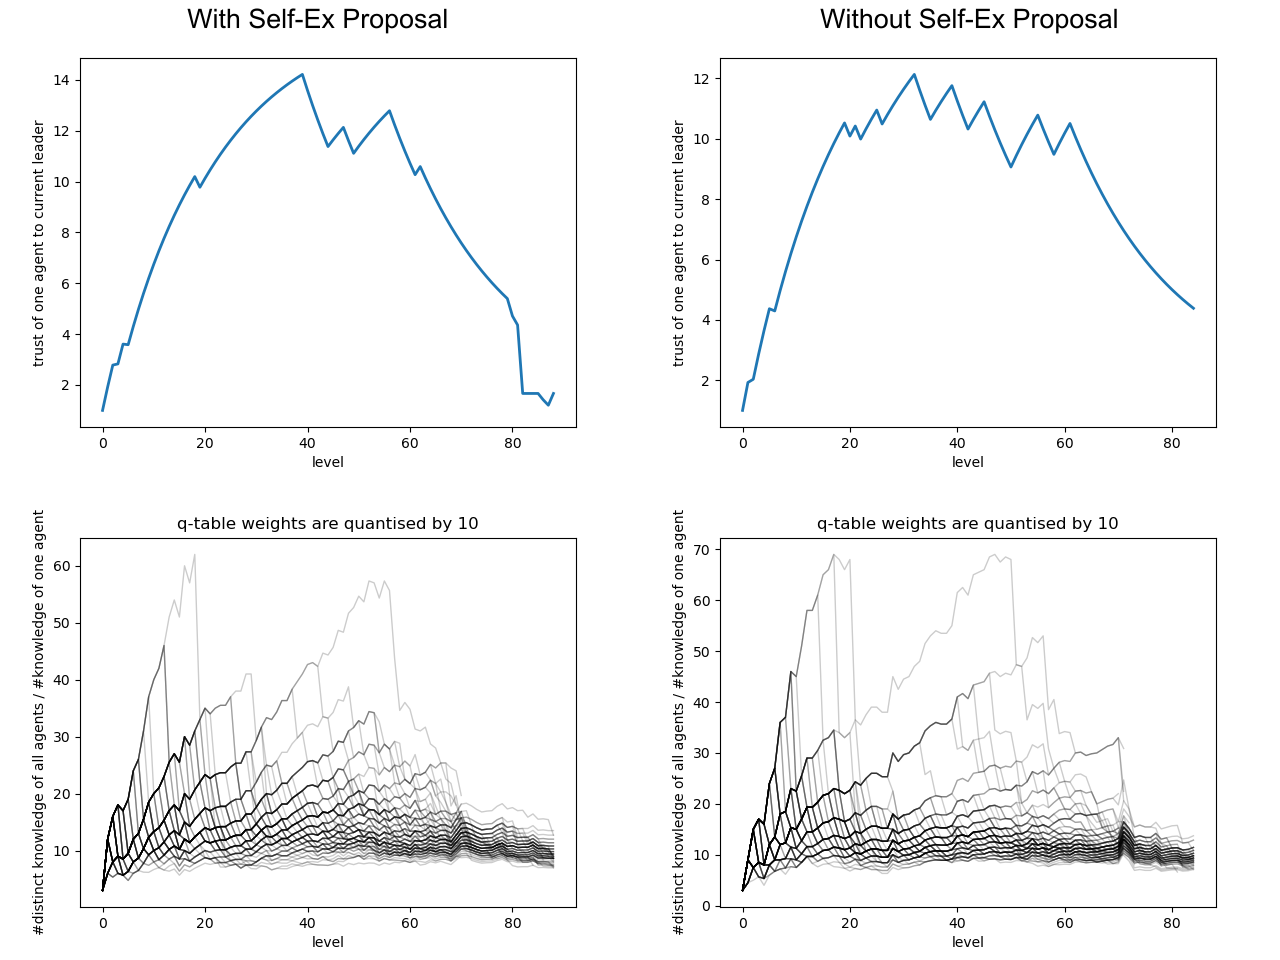
\includegraphics[width=0.8\textwidth]{008_team_5_agent_design/images/knowledgeAgg.png}
    \caption{Comparisons of allowing agent proposal or not. Top: agent's trust to the current leader through levels; Bottom: ratio of population knowledge to individual knowledge through levels.}
    \label{fig:knowledgeAgg}
\end{figure}

For the top part of figure \ref{fig:knowledgeAgg}, we compared how proposal affects leading. Notice that without self-experience proposal, an agent's trust toward the current leader oscillates much frequently. This could infer more repeat leader change, also could be seen as an evidence for higher dependency on the leader.

For the bottom part of figure \ref{fig:knowledgeAgg}, we compared how proposal affects change of the population to individual knowledge ratio. In both cases, the ratio generally increases through the early part of the game, indicating the population knowledge base is growing in a much faster rate than each individual's, but start to drop at mid-game and finally converges. The one with proposal has more variations on how the ratio changes, resulting in more dense spaces between curves. This could reflect that the agents are trying to gain extract knowledge by accepting proposals from others.
